% ==============================================================================
% presentation.tex -- 15-minute Beamer deck
% Paper: "Capping the Capacity Market: A Supply Function Equilibrium Analysis
%        of Price Controls in PJM"
%
% Compile (3-pass pdflatex, from Slides/ directory):
%   pdflatex -interaction=nonstopmode presentation.tex
%   pdflatex -interaction=nonstopmode presentation.tex
%   pdflatex -interaction=nonstopmode presentation.tex
% ==============================================================================

\documentclass[aspectratio=169,14pt]{beamer}

\usetheme{metropolis}
\usepackage[T1]{fontenc}
\usepackage[sfdefault]{FiraSans}
\usepackage{amsmath,amssymb}
\usepackage{booktabs}
\usepackage{tikz}
\usepackage{graphicx}
\usetikzlibrary{positioning,arrows.meta}

% --- Metropolis color accents from paper palette ---
\definecolor{primaryDark}{HTML}{2c3e50}
\definecolor{primaryBlue}{HTML}{2980b9}
\definecolor{accentRed}{HTML}{c0392b}

\setbeamercolor{frametitle}{bg=primaryDark, fg=white}
\setbeamercolor{alerted text}{fg=accentRed}
\setbeamercolor{progress bar}{fg=primaryBlue, bg=primaryDark!20}

% Graphics path
\graphicspath{{../Figures/}}

% Title page metadata
\title{Capping the Capacity Market}
\subtitle{A Supply Function Equilibrium Analysis of Price Controls in PJM}
\author{}
\institute{}
\date{\today}

% ==============================================================================
\begin{document}
% ==============================================================================

% ---------- 1. Title ----------
\maketitle

% ---------- 2. The $21B puzzle ----------
\begin{frame}{The \$21 Billion Question}
  \begin{itemize}
    \item \textbf{Dec 2024:} Pennsylvania files FERC complaint after the
          2025/26 auction clears at \$269.92/MW-day (+800\%{} YoY).
    \item \textbf{Jan 2025:} Shapiro--PJM settlement caps the 2026/27 and
          2027/28 auctions at \textbf{\$325} with a \textbf{\$175} floor.
    \item \textbf{The claim:} over \textbf{\$21 billion} in two-year consumer
          savings.
  \end{itemize}
\end{frame}

% ---------- 3. Research Question ----------
\begin{frame}{Research Question}
  \vfill
  \begin{center}
    \Large
    What would PJM's 2026/27 and 2027/28 auctions have cleared at
    \textbf{absent the settlement}? \\[1em]
    And what is the actual revenue transfer it produces?
  \end{center}
  \vfill
\end{frame}

% ---------- 4. PJM's VRR demand curve ----------
\begin{frame}{The VRR Demand Curve}
  \begin{columns}[T,onlytextwidth]
    \column{0.55\textwidth}
    \begin{center}
      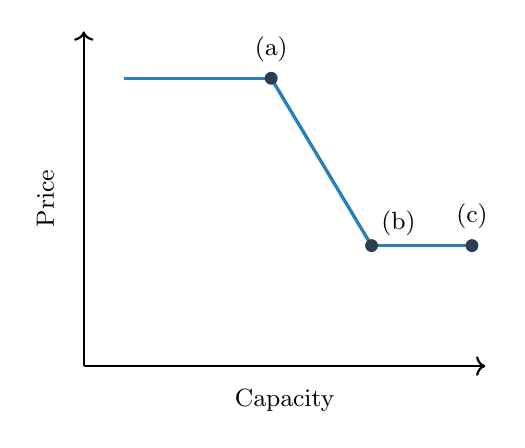
\begin{tikzpicture}[scale=0.85]
        \draw[->, thick] (0,0) -- (6.0,0);
        \node[below] at (3.0,-0.2) {\small Capacity};
        \draw[->, thick] (0,0) -- (0,5.0);
        \node[rotate=90, above] at (-0.3,2.5) {\small Price};
        \draw[primaryBlue, very thick] (0.6,4.3) -- (2.8,4.3);
        \draw[primaryBlue, very thick] (2.8,4.3) -- (4.3,1.8);
        \draw[primaryBlue, very thick] (4.3,1.8) -- (5.8,1.8);
        \filldraw[primaryDark] (2.8,4.3) circle (2.5pt);
        \node[above] at (2.8,4.4) {\small (a)};
        \filldraw[primaryDark] (4.3,1.8) circle (2.5pt);
        \node[above right] at (4.3,1.8) {\small (b)};
        \filldraw[primaryDark] (5.8,1.8) circle (2.5pt);
        \node[above] at (5.8,1.9) {\small (c)};
      \end{tikzpicture}
    \end{center}

    \column{0.42\textwidth}
    \begin{itemize}
      \item Price falls as committed capacity rises.
      \item Flat above (a): admin.\ cap.
      \item Slope (a)--(b): scarcity region.
      \item Flat below (b): excess supply.
    \end{itemize}
  \end{columns}
\end{frame}

% ---------- 5. Settlement as overlay ----------
\begin{frame}{The Settlement as Cap + Floor}
  \begin{columns}[T,onlytextwidth]
    \column{0.55\textwidth}
    \begin{center}
      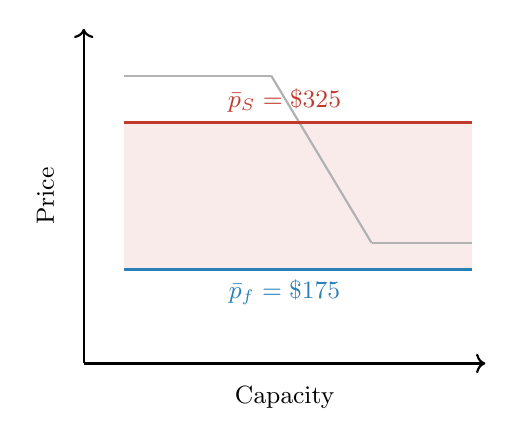
\begin{tikzpicture}[scale=0.85]
        \draw[->, thick] (0,0) -- (6.0,0);
        \node[below] at (3.0,-0.2) {\small Capacity};
        \draw[->, thick] (0,0) -- (0,5.0);
        \node[rotate=90, above] at (-0.3,2.5) {\small Price};
        \fill[accentRed!10] (0.6,1.4) rectangle (5.8,3.6);
        \draw[gray!60, thick] (0.6,4.3) -- (2.8,4.3);
        \draw[gray!60, thick] (2.8,4.3) -- (4.3,1.8);
        \draw[gray!60, thick] (4.3,1.8) -- (5.8,1.8);
        \draw[accentRed, very thick] (0.6,3.6) -- (5.8,3.6);
        \node[accentRed, above] at (3.0,3.6) {\small $\bar{p}_S = \$325$};
        \draw[primaryBlue, very thick] (0.6,1.4) -- (5.8,1.4);
        \node[primaryBlue, below] at (3.0,1.4) {\small $\bar{p}_f = \$175$};
      \end{tikzpicture}
    \end{center}

    \column{0.42\textwidth}
    \begin{itemize}
      \item Cap at \textbf{\$325} truncates from above.
      \item Floor at \textbf{\$175} supports from below.
      \item 2026/27 and 2027/28 only, RTO + constrained LDAs.
    \end{itemize}
  \end{columns}
\end{frame}

% ---------- 6. Model setup ----------
\begin{frame}{Model: Supply Function Equilibrium}
  $K$ symmetric strategic sellers bid supply functions against PJM's VRR
  demand. Following Klemperer \& Meyer (1989):
  \vfill
  \begin{equation*}
    s'(p) \;=\; \frac{D'(p) \,+\, s(p)/(p - c)}{K - 1}
  \end{equation*}
  \vfill
  \begin{itemize}
    \item Boundary: $s(\bar{p}) = \bar{q}$ \hfill (Holmberg 2008)
    \item Fringe: competitive block $Q_f$ offered at cost $c$.
    \item Equilibrium price $p^*$: where $K\cdot s(p^*) + Q_f = D(p^*)$.
  \end{itemize}
\end{frame}

% ---------- 7. At-cap is mechanical ----------
\begin{frame}{The At-Cap Regime Is Mechanical}
  \begin{itemize}
    \item When $K \leq 3$, the interior ODE cannot clear demand below $\bar{p}$.
    \item Market then clears at $\bar{p}$ by construction.
    \item The dollar value is read off PJM's planning parameters, not
          predicted by the model.
  \end{itemize}
  \vfill
  \begin{center}
    \alert{The substantive content is the \textit{regime}
    (at-cap vs.\ interior) and its dependence on $K$.}
  \end{center}
\end{frame}

% ---------- 8. Calibration ----------
\begin{frame}{Calibration}
  \begin{itemize}
    \item \textbf{$K = 3$} strategic sellers --- all seven BRA years show
          RSI$_3 < 1$ at the RTO level.
    \item \textbf{$c = \$150$/MW-day} --- combined-cycle sector ACR
          (IMM 2025).
    \item \textbf{VRR curve, demand, CETL} from PJM planning filings.
  \end{itemize}
\end{frame}

% ---------- 9. Baseline results ----------
\begin{frame}{Baseline SFE Equilibrium}
  \begin{center}
    \small
    \begin{tabular}{lcccc}
      \toprule
      Year & Design & $p^*$ & Actual & Outcome \\
      \midrule
      2021/22 & Old & \$405 & \$140 & Interior \\
      2022/23 & Old & \$310 & \$50  & Interior \\
      2023/24 & Old & \$330 & \$34  & Interior \\
      2024/25 & Old & \$358 & \$29  & Interior \\
      2025/26 & Old & \$426 & \$270 & Interior \\
      \midrule
      \textbf{2026/27} & \textbf{New} & \textbf{\$329} & \textbf{\$329} & \textbf{At cap} \\
      \textbf{2027/28} & \textbf{New} & \textbf{\$333} & \textbf{\$333} & \textbf{At cap} \\
      \bottomrule
    \end{tabular}
  \end{center}
  \vspace{0.4em}
  \footnotesize Old-design gaps reflect unmodeled TPS mitigation.
\end{frame}

% ---------- 10. Key finding: K transition ----------
\begin{frame}{Markups Collapse Between $K = 3$ and $K = 4$}
  \begin{center}
    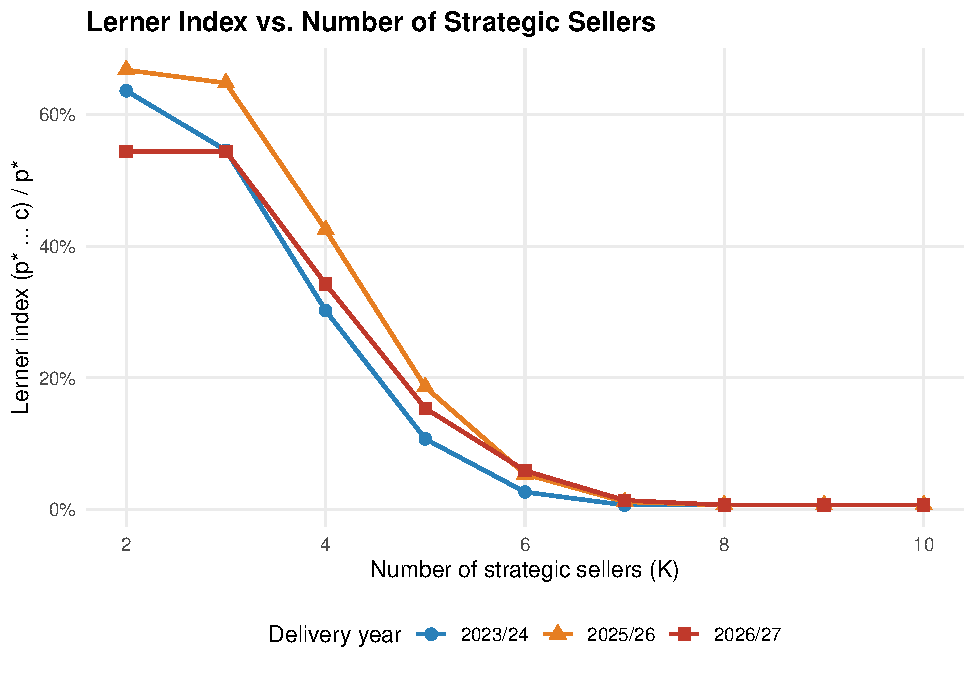
\includegraphics[height=0.75\textheight]{fig02b_K_lerner.pdf}
  \end{center}
\end{frame}

% ---------- 11. The $21B reassessment ----------
\begin{frame}{The \$21 Billion, Reassessed}
  \begin{center}
    \small
    \begin{tabular}{lccc}
      \toprule
      Counterfactual & 2026/27 & 2027/28 & Two-year total \\
      \midrule
      VRR Point~(a) [Shapiro] & \$500 & \$500 & \textbf{\$17.16B} \\
      SFE equilibrium [this paper] & \$329 & \$333 & \textbf{\$0.61B} \\
      \midrule
      Settlement cap & \$325 & \$325 & --- \\
      \bottomrule
    \end{tabular}
  \end{center}
  \vspace{1em}
  \begin{center}
    \alert{Same arithmetic. Different counterfactual.}
  \end{center}
\end{frame}

% ---------- 12. Limitations ----------
\begin{frame}{Limitations}
  \begin{itemize}
    \item \textbf{TPS mitigation} not modeled endogenously --- may be the
          true binding constraint absent the settlement.
    \item \textbf{Symmetric firms} --- cost heterogeneity bracketed,
          not solved.
    \item \textbf{$K = 3$ imposed at LDA level} where RSI data is sparse.
    \item \textbf{Static model} --- no retirement or entry response to
          suppressed prices.
  \end{itemize}
\end{frame}

% ---------- 13. Implications & Conclusion ----------
\begin{frame}{What the Settlement Does --- and What It Doesn't}
  \begin{itemize}
    \item The cap \textbf{truncates the price signal};
          it does not alter the conditions that place the
          equilibrium there.
    \item Three structural channels --- \textbf{transmission},
          \textbf{VRR slope}, \textbf{entry} --- reduce markups
          without truncating the signal.
    \item Temporary price suppression is not a substitute for
          structural reform.
  \end{itemize}
  \vfill
  \begin{center}
    \large Thank you.
  \end{center}
\end{frame}

\end{document}
